\documentclass[10pt,twocolumn]{article}

\usepackage[a4paper,margin=2cm,columnsep=0.7cm]{geometry}
\usepackage{amsmath,amssymb}
\usepackage{graphicx}
\usepackage{booktabs}
\usepackage{microtype}
\usepackage[numbers,sort&compress]{natbib}
\usepackage[font=small,labelfont=bf]{caption}
\usepackage{xcolor}
\usepackage[hidelinks]{hyperref}

\graphicspath{{../results/figures/stage3_mechanism/}{../results/figures/stage4_integration/}}

% Draft helper; remove before submission.
\newcommand{\todo}[1]{\textcolor{red}{[TODO: #1]}}

\title{\textbf{Accelerating ColBERT MaxSim with BOND-Style Dimension Pruning on a PDX Layout}}
\author{Martan van der Straaten\\Radboud University\\\texttt{martanvanderstraaten@gmail.com}}
\date{\today}

\begin{document}
\maketitle

\begin{abstract}
ColBERT scores documents with late interaction: every query token is compared
against every document token, which makes exact retrieval expensive. BOND
showed, for single-vector search on a vertically decomposed layout, that
scanning dimensions incrementally and pruning candidates with a partial-score
bound can skip most of this work. In this paper, we investigate whether that
idea transfers to ColBERT's MaxSim operator on the modern PDX layout, on a
single CPU node. We formalize the bound for MaxSim, prove it exact-safe, and
implement it in a fused vectorized kernel whose dense variant already
outperforms an OpenBLAS baseline by roughly $3\times$. We find that the
mechanism transfers only partially: the Cauchy--Schwarz bound stays too loose
to prune anything until late in the dimension scan, so early pruning never
pays for its bookkeeping. Pruning at late checkpoints does discard
88--98\% of documents exactly, but at that point most of the memory
traffic has already been paid, and the wall-clock win over our own dense
baseline is decisive on only one of four datasets. \todo{finalize abstract
once Stage 4 results are frozen}
\end{abstract}

\section{Introduction}
\label{sec:intro}

Neural retrieval models rank documents by comparing dense vector
representations of queries and documents. ColBERT~\cite{khattab2020colbert}
takes a fine-grained approach: instead of one vector per document, it keeps
one vector per \emph{token}, and scores a query--document pair with late
interaction,
\begin{equation}
  \mathrm{score}(q, d) \;=\; \sum_{i} \max_{j} \,\langle q_i, d_j \rangle ,
  \label{eq:maxsim}
\end{equation}
the sum over query tokens of the best-matching document token. This MaxSim
operator is more accurate than single-vector retrieval, but it is also much
more expensive: a query with $m$ tokens against a corpus of $N$ token vectors
costs $m \times N$ inner products of dimension $D$. Production systems avoid
this cost with approximate indexes such as PLAID~\cite{santhanam2022plaid},
which trade exactness for speed. We are interested in a different lever:
can we keep the result \emph{exact} and still skip most of the work?

BOND~\cite{devries2002bond} offers a candidate mechanism. On a vertically
decomposed (column-per-dimension) layout, it scans dimensions incrementally,
maintains a partial score per candidate, and discards a candidate as soon as
an upper bound on its final score falls below the current top-$k$ threshold.
The recent PDX layout~\cite{kuffo2025pdx} revives this vertical design for
modern SIMD hardware and shows large speedups for single-vector search. Both
results are for one query vector and one score per candidate. MaxSim breaks
both assumptions: there are $m \approx 21$ query tokens, and the score is a
sum of maxima over a variable-length set of document tokens. Whether
dimension pruning survives this change is not obvious, and that is the
question of this paper.

\subsection{Research questions}

Our primary research question is:

\begin{quote}
\textbf{Can a PDX-compatible implementation of BOND-style dimension pruning
accelerate ColBERT MaxSim retrieval at matched retrieval quality on a single
CPU node?}
\end{quote}

We decompose it into four subquestions:

\begin{itemize}
  \item \textbf{RQ1 (mechanism).} How much work can a valid MaxSim bound
    save in principle, and where in the dimension scan does pruning become
    possible?
  \item \textbf{RQ2 (baseline).} What is the strongest honest dense MaxSim
    baseline on this hardware, and does the PDX layout itself matter in the
    MaxSim regime?
  \item \textbf{RQ3 (exact-safe gate).} Does exact-safe BOND pruning beat
    that dense baseline in wall-clock time?
  \item \textbf{RQ4 (system).} How does the pruned kernel compose with
    candidate generation (IVF, PLAID), compared fairly at fixed candidate
    budgets?
\end{itemize}

We answer RQ1 with accounting instruments that measure bound tightness and
candidate survival independently of any implementation, RQ2 and RQ3 with a
purpose-built fused kernel measured against its own dense variant, and RQ4
with an integration study in which every method is timed end-to-end on the
same machine at the same candidate budget. The approximate regime, where the
bound is deliberately shrunk below its safe value, is out of scope for this
paper; we return to it in the discussion.

\subsection{Contributions}

The contributions of this paper are the following:

\begin{itemize}
  \item We formalize BOND-style dimension pruning for MaxSim and prove the
    resulting method exact-safe, at both the document and the token level,
    including its transfer to a checkpointed, panel-blocked kernel.
  \item We design a fused MaxSim kernel on the PDX layout that outperforms a
    multithreaded OpenBLAS dense baseline by roughly $3\times$. This kernel
    is a standalone contribution, independent of pruning.
  \item We explain \emph{why} the BOND mechanism largely fails for MaxSim:
    the Cauchy--Schwarz envelope stays wider than ColBERT's score gaps until
    roughly 75\% of the dimensions are paid for. Late-checkpoint pruning is
    the one operating point where the mechanism fires.
  \item We contribute a measurement methodology, interleaved baseline timing
    and fixed candidate budgets, that corrected two of our own headline
    numbers and one circulating external comparison.
\end{itemize}

The remainder of this paper is structured as follows. Section~\ref{sec:background}
covers the background: late interaction, BOND, and the PDX layout.
Section~\ref{sec:design} presents our formalization and kernel designs.
Section~\ref{sec:method} describes the experimental setup and how each
experiment answers a research question. Section~\ref{sec:results} presents
the results, and Section~\ref{sec:discussion} discusses and concludes.

\section{Background}
\label{sec:background}

In this section, we briefly cover the three research lines this paper builds
on, and the baseline systems we compare against.

\subsection{ColBERT and late interaction}

Dense retrieval encodes queries and documents as vectors and ranks by vector
similarity. Single-vector models compress each document into one embedding,
which is cheap to search but lossy. ColBERT~\cite{khattab2020colbert} instead
keeps one embedding per token and defers the interaction between query and
document to search time, through the MaxSim score of
Equation~\ref{eq:maxsim}: each query token picks the document token that
matches it best, and the document's score is the sum of these best matches.
All token embeddings are unit-normalized, so each inner product is a cosine
similarity. Late interaction retains much of the effectiveness of full
cross-attention rerankers while keeping document representations precomputable
\cite{santhanam2022colbertv2}. The price is scoring cost: the corpus holds an
order of magnitude more vectors ($N$ tokens rather than $N$ documents), and
every query token must visit all of them for an exact result.

\subsection{BOND: dimension-incremental pruning}

BOND~\cite{devries2002bond} accelerates exact nearest-neighbor search on a
vertically decomposed store: values are grouped by \emph{dimension}, not by
vector, so the engine can scan dimension 1 of every candidate, then dimension
2, and so on. After scanning a prefix of dimensions, every candidate has a
partial score, and a bound on what the unscanned remainder can still
contribute. A candidate whose optimistic bound cannot reach the current
$k$-th best score is discarded without reading its remaining values.
Correctness is immediate as long as the bound is a true upper bound, which
makes the method \emph{exact-safe}: it returns exactly the top-$k$ of a full
scan. The appeal is that the threshold rises as good candidates finish, so
later candidates are pruned earlier; the risk is that the bound is loose, in
which case nothing is pruned and the bookkeeping is pure overhead. Notably,
the original paper reports that for L2 search a \emph{cheap} query-side bound
beat their tighter bound at wall-clock, because the tighter bound's
bookkeeping did not pay off. We will revisit exactly this trade-off for
MaxSim.

\subsection{The PDX layout}

PDX~\cite{kuffo2025pdx} is a recent data layout for vector similarity search
that decomposes vectors \emph{within blocks}: inside a block of vectors,
values are stored dimension-major, so a SIMD register can process one
dimension of many candidates at once. This gives distance kernels that
auto-vectorize cleanly, and it makes dimension-incremental pruners such as
BOND and ADSampling~\cite{gao2023adsampling} natural to express: pruning a
candidate means masking a lane, and stopping early means not loading the
remaining dimension columns at all. The published PDX results are, like BOND,
for single-vector queries ($m = 1$): each corpus value is loaded, used in one
multiply-add, and discarded, so the workload is memory-bound and layout plus
pruning are the only levers. An important observation for this paper is that
MaxSim changes this regime: with $m \approx 21$ query tokens, every loaded
document value is reused $m$ times, which moves the workload from the
GEMV regime toward GEMM, where register blocking and operand reuse dominate.
A pruning mechanism therefore has to beat a much stronger dense baseline than
in the published $m = 1$ setting.

\subsection{Candidate generation baselines}

The alternative to scanning the full corpus is generating a small candidate
set first. IVF indexes cluster the corpus and probe only the nearest
clusters at query time; we use the FAISS implementation~\cite{douze2024faiss}
with an exact MaxSim rerank on top, aggregating per-token search hits into
document candidates. PLAID~\cite{santhanam2022plaid} is the ColBERT-native
pipeline, combining centroid-based candidate generation with compressed
scoring stages. Both are approximate: their recall depends on how many
candidates are probed. In our comparisons, all such methods are evaluated at
a \emph{fixed candidate budget}, so a candidate-generation speedup can never
masquerade as a scoring speedup (Section~\ref{sec:method:protocol}).

\section{BOND-MaxSim: bound and kernels}
\label{sec:design}

This section presents our own work: the MaxSim bound and its safety
proof (\ref{sec:design:bound}), the fused dense kernel that serves as the
honest baseline (\ref{sec:design:dense}), the pruned variants built on it
(\ref{sec:design:bond}), and the accounting instruments that let us separate
the mechanism from the implementation (\ref{sec:design:instruments}).

\subsection{The bound, and when pruning is safe}
\label{sec:design:bound}

Let $S$ be the set of dimensions scanned so far (a prefix of a chosen scan
order), and let $P_{ij}(S) = \sum_{z \in S} q_{iz} d_{jz}$ be the partial
inner product of query token $i$ and document token $j$. By Cauchy--Schwarz,
the unscanned remainder is bounded by the product of the residual norms:
\begin{equation}
  \big|\langle q_i, d_j\rangle - P_{ij}(S)\big| \;\le\;
  \underbrace{\|q_i^{S^c}\| \cdot \|d_j^{S^c}\|}_{R_{ij}(S)} ,
\end{equation}
and since all tokens are unit-norm, both residual norms follow from the
scanned energy alone: $\|x^{S^c}\|^2 = 1 - \sum_{z \in S} x_z^2$. Thus every
pair has a valid interval $P_{ij} \pm R_{ij}$ at every prefix, without
touching unscanned values. Summing the upper ends over query tokens gives a
document-level upper bound
\begin{equation}
  \mathrm{score}(q, d) \;\le\; \sum_i \max_j \big( P_{ij}(S) + R_{ij}(S) \big)
  \;=\; \mathrm{UB}_d(S),
  \label{eq:ubd}
\end{equation}
and the BOND pruning rule carries over: if $\mathrm{UB}_d(S) < \tau_k$, the
$k$-th best exact score so far, document $d$ can be discarded. The same
intervals support a \emph{token-level} test inside one document: a document
token can be dropped once it is dominated, for every query token, by some
other token's lower bound. We prove that this never drops any query token's
true argmax (the \emph{survival invariant}), so finalized scores are exact
and, by induction, the returned top-$k$ equals the exact top-$k$. The proof
needs three preconditions: unit-norm tokens, exact arithmetic, and top-$k$
by set equality. Unit normalization deserves emphasis: it is a
\emph{safety} precondition, not a convenience. If a stored norm exceeds~1,
the residual is underestimated and exactness silently breaks, so our
pipeline verifies norms at export time.

The bound also admits an approximate mode that scales the residual down by a
factor $\mathrm{shrink} < 1$, trading recall for pruning. No recall guarantee
survives this, so we treat it as a separate regime and exclude it from this
paper's claims; everything below runs at $\mathrm{shrink} = 1$.

Two further lemmas transfer the proof from the per-document formulation to
the blocked kernel of Section~\ref{sec:design:bond}: a coarser (checkpointed,
document-level) bound is looser than the per-dimension one and therefore
still safe, and padding documents to a fixed token multiple is harmless if
the padding \emph{duplicates a real token}. Zero-padding would not be: a
zero token contributes $\max_j 0 = 0$, which corrupts scores when all true
maxima are negative. On the query side the situation is reversed and
zero-padding is exact. Finally, a threshold shared by all threads only ever
rises toward the true $\tau_k$ from below, so parallel execution stays safe.

\subsection{A fused dense kernel: the honest baseline}
\label{sec:design:dense}

Our first measurements made clear that the interesting engineering question
is not the pruner but the baseline. A straightforward NumPy formulation of
Equation~\ref{eq:maxsim}, one large matrix product $Q X^\top$ followed by a
segmented maximum, runs on all cores of our machine through OpenBLAS, and it
beat our initial columnar scan by $8\times$. Any pruning claim measured
against a weak scan would be meaningless. We therefore built the strongest
dense kernel we could, and it is this kernel that every pruning result in
this paper must beat.

The kernel exploits the observation from Section~\ref{sec:background} that
MaxSim is GEMM-shaped. It packs the corpus once, at build time, into
panel-major PDX blocks: panels of 16 document tokens stored dimension-major,
documents padded to a panel multiple by duplicating their last token. At
query time an AVX-512 register tile accumulates all $m$ query tokens against
one panel across the dimension range, and the per-document maximum is folded
in registers as each document's last panel completes, so the $m \times N$
score matrix is never materialized. This removes the three costs that BLAS
cannot avoid: re-packing the operand on every call, writing the full score
matrix, and reading it back for the reduction. The result is a kernel that
computes the identical exact scores at roughly $3\times$ the speed of the
12-thread OpenBLAS formulation, and roughly $2\times$ single-threaded.

\subsection{Fused BOND kernels}
\label{sec:design:bond}

The pruned variant keeps the identical microkernel and adds pruning at a
small set of \emph{checkpoints} $C \subseteq \{1,\dots,D\}$: it processes one
document at a time depth-first across dimension segments, and at each
checkpoint evaluates $\mathrm{UB}_d$ (Equation~\ref{eq:ubd}) against a shared,
rising threshold $\tau$. If the document survives all checkpoints, the final
segment folds its exact score as in the dense kernel. Because pruning is the
only difference to the dense arm, any wall-clock gap between the two is
attributable to the mechanism, not to implementation drift; the two arms
produce bit-identical scores for unpruned documents, which our test suite
verifies on every dataset. Three variants exist: a document-level arm, a
token-level arm that additionally applies the domination test of
Section~\ref{sec:design:bound} with lane masking, and a \emph{cheap-bound}
arm that relaxes the document-side residual to 1, mirroring the query-only
bound the original BOND paper found superior for L2. The checkpoint set $C$
and the threshold policy (self-seeded, externally seeded, or an oracle
threshold for accounting) are parameters throughout.

The threshold can also be \emph{seeded}: any lower bound on the true
$\tau_k$ is safe, and a better starting threshold means earlier pruning. Our
seeded arm obtains candidates from a small IVF probe and scores a handful of
them exactly before the scan starts. On top of this we build one approximate
system arm, the \emph{partitioned fused scan}: documents are clustered at
build time, each cluster is packed in panel layout, and a query probes only
its nearest clusters with the fused kernel as the in-cluster scanner. This
is the PDX-IVF architecture with our kernel inside; unlike everything else
above it can miss true top-$k$ documents, so it is reported strictly as a
recall--latency frontier.

\subsection{Measurement instruments}
\label{sec:design:instruments}

Wall-clock alone cannot answer RQ1, because a kernel conflates what the
bound \emph{could} prune with what its schedule manages to capture. We keep
three instruments separate from the throughput kernels. First, a wide-block
\emph{accounting} kernel evaluates both pruning tests at every dimension
fetch, breadth-first over a block of tokens, and counts exactly which cells
of the (token $\times$ dimension) grid are touched: this is the upper
envelope of what any schedule could save, the mechanism under a microscope.
Second, a NumPy \emph{checkpoint simulator} replays the fused kernel's
document-level policy at a fixed threshold and predicts its pruning and cell
counts; we validate it against the kernel's own counters. Third, the exact
NumPy oracle provides ground-truth scores, and every exact-safe run is gated
on exact top-$k$ agreement with it (ties at the $k$-th rank are accepted by
score). Accounting numbers (cells touched) and wall-clock numbers are never
mixed in what follows: the former answer RQ1, the latter RQ3.

\section{Methodology}
\label{sec:method}

\subsection{Setup}
\label{sec:method:setup}

\paragraph{Data and embeddings.} We evaluate on four BEIR
corpora~\cite{thakur2021beir}: NFCorpus (3{,}633 documents), SciFact
(5{,}183), ArguAna (8{,}674), and SciDocs (25{,}657). Documents and queries
are embedded with GTE-ModernColBERT-v1 through PyLate~\cite{chaffin2024pylate}
($D = 128$, unit-norm token vectors; SciFact yields about 1.1M token
vectors). Each experiment uses a fixed 50-query subsample (seed 42) and
retrieves the top $k = 10$. Retrieval quality for exact-safe arms is
exact agreement with the oracle; approximate arms report recall@10 against
the same oracle.

\paragraph{Hardware.} All measurements run on one machine: an AMD Zen~5
laptop CPU (Ryzen AI 7 445, 6 cores / 12 threads, AVX-512, 1\,MB L2 per
core) under Fedora Linux. Kernels are C++ compiled with GCC and called
through ctypes; the dense external reference is NumPy with
scipy-openblas 0.3.31. Every arm is measured both single-threaded and on
all cores, and thread counts are always reported with the number.

\subsection{Measurement protocol}
\label{sec:method:protocol}

Fair timing turned out to be a research problem of its own, and two controls
in particular decide our conclusions.

\paragraph{Interleaved baselines.} Comparing a candidate arm against a dense
baseline timed in a separate run is not safe on a laptop-class CPU: thermal
and frequency state drift between runs. We time all arms
\emph{interleaved}, round-robin in one process, best-of-5 per arm. This
control corrected our own headline number: a standalone-timed baseline had
inflated one dataset's pruning win from $+8.7\%$ to $-19.6\%$.

\paragraph{Fixed candidate budgets.} When comparing candidate-generation
methods (RQ4), every method is granted the same budget $B$ of documents
eligible for full scoring, with $B$ on the axis. A method may fill its
budget with better candidates and win on recall, but it cannot win the
latency comparison by silently scoring fewer documents. Complete pipelines
sit inside the timer, including per-token hit aggregation, and index build
cost is reported separately from query latency. We adopted this control
after dissecting an earlier exploratory benchmark of these systems, in which
a $164\times$ budget mismatch, an untimed pipeline stage, and two different
runtime stacks compounded into headline speedups that do not survive
matched conditions.

\paragraph{Separation of regimes.} Exact-safe and approximate results never
share a table: exact-safe arms must pass the exact-agreement gate, and
approximate arms live on recall--latency frontiers. Similarly, accounting
(cells touched) and wall-clock are produced by different instruments and
reported apart.

\subsection{Experiments}
\label{sec:method:experiments}

Table~\ref{tab:experiments} maps the experiments to the research questions.
The mechanism experiments (RQ1) measure the bound itself: e01 measures bound
slack, the ratio $\mathrm{UB}_d / \mathrm{score}$, as a function of scan
depth; e02 measures survival curves, the fraction of documents and tokens
still alive at each depth under three threshold policies (self-seeded,
seeded, oracle) and three dimension orders (natural, BOND's
variance-descending order, PCA rotation). The kernel experiments (RQ2, RQ3)
compare the fused dense arm against NumPy/OpenBLAS and against the fused
BOND arms across orders and granularities (e03), checkpoint sets (e08), and
the tight versus cheap bound (e09), all at $\mathrm{shrink}=1$ under the
interleaved protocol. The integration experiments (RQ4) compare, at fixed
budgets, the exhaustive fused scan, seeded exact-safe BOND, FAISS-IVF with
exact rerank, PLAID, and the partitioned fused scan (s01); ablate what a
realistic IVF seed recovers of the oracle threshold's pruning (s02); and
sweep the partitioned arm's probe count as a recall--latency frontier (s03).

Each experiment writes one shared result schema (dataset, arm, thread count,
timing, pruning statistics, quality gate) to versioned JSON, and every
figure in Section~\ref{sec:results} is generated from those files.

\begin{table}[t]
\centering
\small
\begin{tabular}{@{}lll@{}}
\toprule
RQ & Experiments & Instrument \\
\midrule
RQ1 & e01 bound slack; e02 survival & accounting kernel \\
RQ2 & dense arm vs.\ OpenBLAS (e03) & fused kernel \\
RQ3 & e03 orders; e08 checkpoints; & fused kernel, \\
    & e09 bound tightness & interleaved \\
RQ4 & s01 fixed-budget arms; s02 seeds; & full pipelines, \\
    & s03 partitioned frontier & interleaved \\
\bottomrule
\end{tabular}
\caption{Experiments per research question. Stage-3 mechanism experiments
are prefixed e, Stage-4 integration experiments s.}
\label{tab:experiments}
\end{table}

\section{Results}
\label{sec:results}

\todo{This section is a skeleton; runs for Stage 4 are still landing. The
RQ1/RQ3 figures below are final.}

\subsection{RQ1: the bound is loose until late in the scan}

\begin{figure}[t]
  \centering
  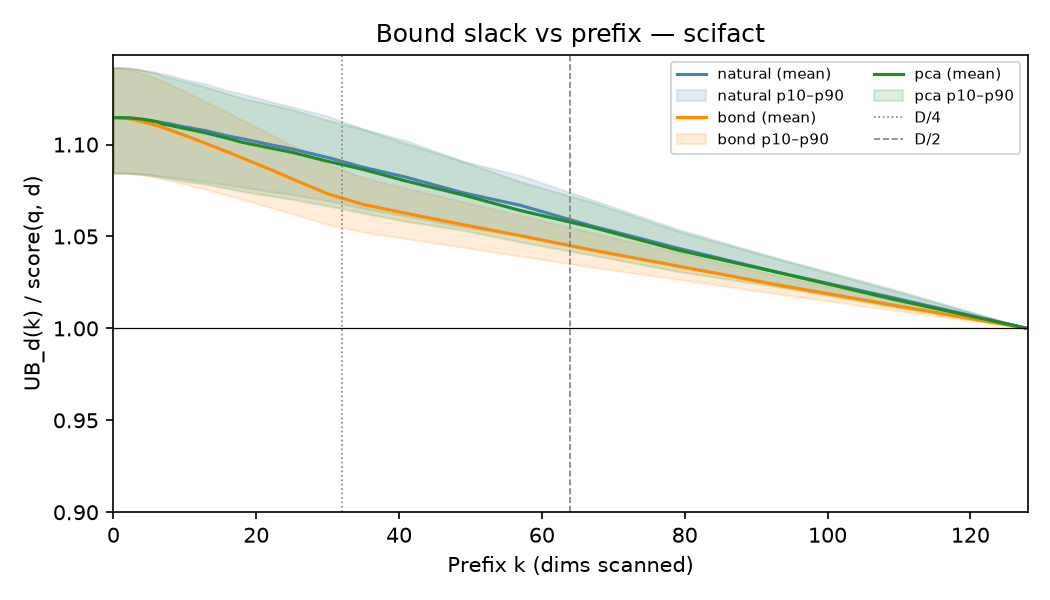
\includegraphics[width=\linewidth]{e01_bound_slack_scifact}
  \caption{Bound slack $\mathrm{UB}_d/\mathrm{score}$ versus scan depth on
  SciFact, for three dimension orders (mean and p10--p90 band over
  query--document pairs). Even at half the dimensions the bound still
  overestimates scores by ${\sim}5\%$, far wider than typical
  inter-document score gaps.}
  \label{fig:e01}
\end{figure}

\begin{figure}[t]
  \centering
  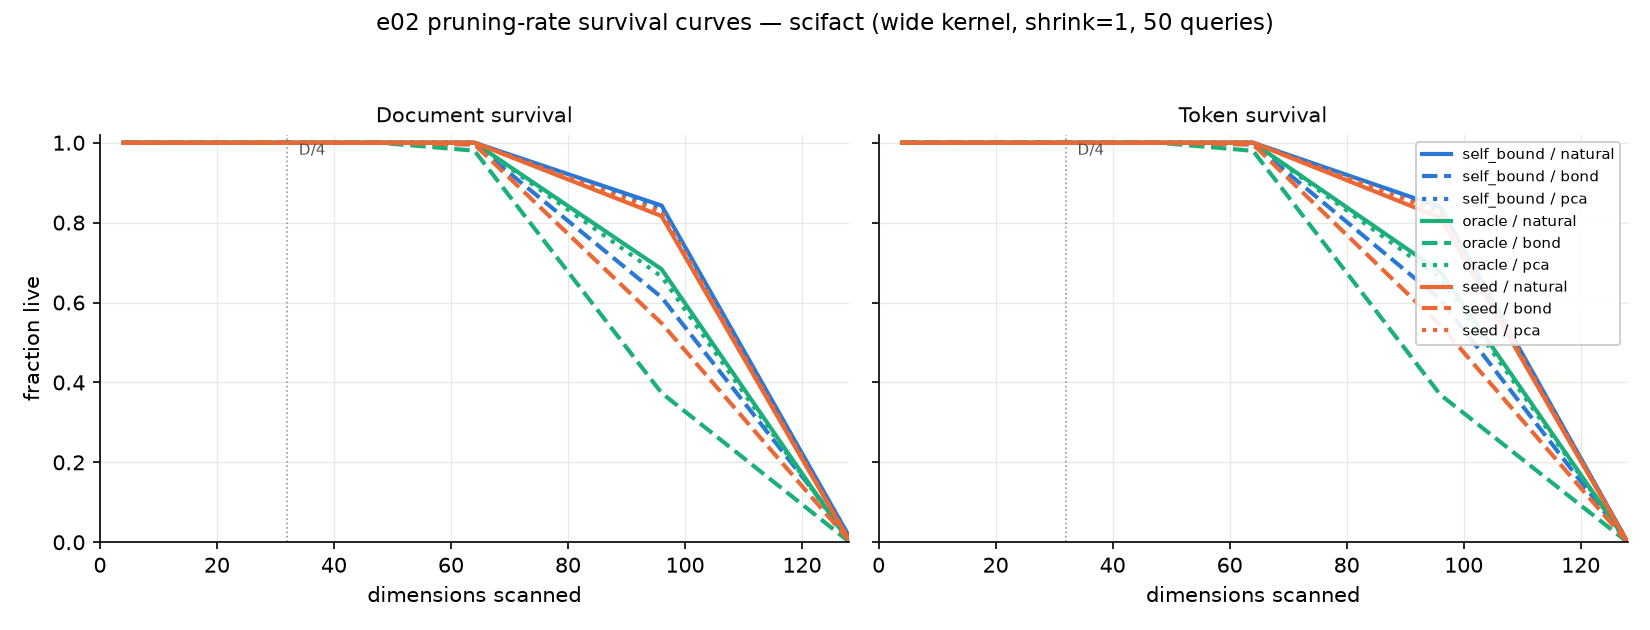
\includegraphics[width=\linewidth]{e02_pruning_rate_scifact}
  \caption{Survival curves on SciFact: fraction of documents (left) and
  tokens (right) still alive versus dimensions scanned, per threshold policy
  and dimension order. Nothing is prunable before dimension 64 of 128; most
  pruning becomes possible only past dimension 96.}
  \label{fig:e02}
\end{figure}

Figures~\ref{fig:e01} and~\ref{fig:e02} answer RQ1. \todo{one paragraph:
slack ${\sim}11\%$ at start, ${\sim}5\%$ at $D/2$; 98--100\% of documents and
tokens unprunable at dimension 64 under every policy and order; accounting
cells 84--92\%, so the exact-safe ceiling is ${\le}16\%$ of work.}

\subsection{RQ2/RQ3: kernels}

\begin{figure}[t]
  \centering
  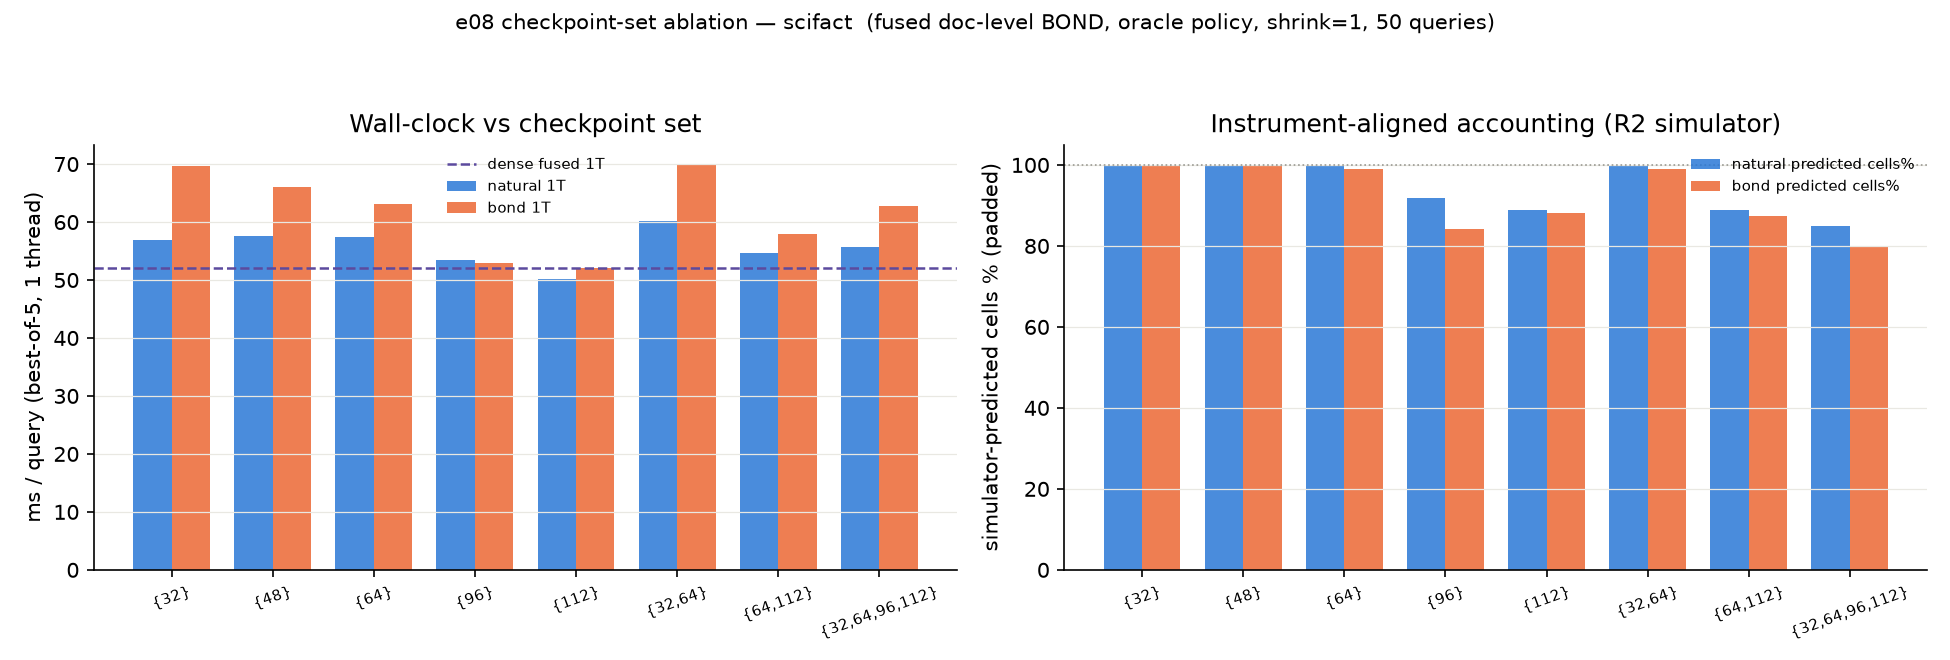
\includegraphics[width=\linewidth]{e08_checkpoint_ablation_scifact}
  \caption{Checkpoint-set ablation on SciFact (single thread, oracle
  threshold). Early checkpoint sets cost more than they save; only late
  single checkpoints ($C = \{96\}, \{112\}$) approach or beat the dense
  baseline (dashed).}
  \label{fig:e08}
\end{figure}

\todo{dense kernel table (1T / all cores, per dataset) vs OpenBLAS; e03
verdict at default checkpoints; e08 late-checkpoint result (88--98\% of
documents pruned exact-safe, recall 1.0); e09 tight-vs-cheap reversal of the
BOND 2002 lesson; interleaved-corrected margins: ArguAna $+8.7\%$, others
within $+0.9$--$2.3\%$.}

\subsection{RQ4: integration}

\todo{s01 fixed-budget figure and discussion (exhaustive fused scan beats
every candidate pipeline at these corpus sizes except SciDocs); s02 seeded
threshold recovers up to 99\% of oracle pruning but seed cost eats the
margin; s03 partitioned frontier.}

\section{Discussion and conclusion}
\label{sec:discussion}

\todo{Answer the four RQs in order; negative-result framing for RQ3 (the
mechanism fails in the bound math, not the engineering); the fused dense
kernel and the measurement methodology as the standing contributions;
limitations (corpus scale, one embedding model, laptop CPU); future work
(approximate shrink frontier, larger corpora, int8/VNNI headroom, CoRECT
IR-quality evaluation).}

\bibliographystyle{unsrtnat}
\bibliography{references}

\end{document}
